\documentclass[a4paper,11pt]{article}

% Identificação
\newcommand{\pbtitulo}{Jenkins}
\newcommand{\pbversao}{1.0}

\usepackage{../sty/tutorial}

%----------------------------------------------------------------------
% Início do Documento
%----------------------------------------------------------------------
\begin{document}
	
\maketitle % mostrar o título
\thispagestyle{fancy} % habilitar o cabeçalho/rodapé das páginas

%----------------------------------------------------------------------
% RESUMO DO ARTIGO
%----------------------------------------------------------------------

\begin{abstract}	
	\initial{N}ão é a mais intelectual das espécies que sobrevive; também não é a mais forte; mas a espécie que sobrevive é a única capaz de se adaptar melhor às mudanças no ambiente em que se encontra. (C. Megginson, interpretando Charles Darwin). \textbf{Jenkins} é uma poderosa ferramenta de código aberto destinado a executar Integração Contínua criada com a linguagem Java o que está associada a sua portabilidade para os mais diversos sistemas operacionais. Permite executar uma lista predefinida de etapas (denominado de \textit{pipeline}), como por exemplo baixar o código-fonte de um repositório na Web, compilar conforme comandos da linguagem e construir um executável a partir das classes resultantes e publicá-la em um servidor definido. O gatilho para esta execução pode ser baseado em uma hora, um evento ou mesmo inciado por demanda.
\end{abstract}

%----------------------------------------------------------------------
% CONTEÚDO DO ARTIGO
%----------------------------------------------------------------------
\section{Entrega Contínua}
A medida que o número de trabalho a realizar aumenta, torna-se cada vez mais difícil para alguém mantê-los. Especialmente nos casos em que o trabalho é uma simples cópia que foi modificada a partir de um outro trabalho, acaba-se por tornar crucial manter uma determinada consistência. A entrega contínua (\textit{Continuous Delivery} ou \textbf{CD}) é a prática de fornecer um software com mais qualidade e frequência. As práticas de CD podem incluir as seguintes vantagens:
\begin{itemize}
	\item Promoção de código automatizado com qualidade.
	\item Estratégia de ramificação do projeto a ser entregue.
	\item Construções distribuídas e razoavelmente mantidas.
	\item Teste automatizado, distribuído ou paralelo.
	\item Provisionamento de um ambiente completamente atualizado e automatizado.
\end{itemize}

Sendo que um dos componentes fundamentais da CD é a Integração Contínua (\textit{Continuous Integration} ou \textbf{CI}) em funcionamento. E é importante possuirmos um modelo de CI amplamente funcional. Principalmente se podemos considerar os seguintes parâmetros como: \textit{pipeline} de CI codificáveis, automação na geração dos executáveis do projeto e ambientes de construção reproduzíveis com alta disponibilidade.

Um \textit{pipeline} de CI é um conjunto de tarefas sequenciais ou paralelas (às vezes uma combinação de ambas). São configurados através de uma simples interface visual.

CD/CI é um processo no qual todo o trabalho de desenvolvimento se encontra integrado o mais cedo possível. Os artefatos resultantes são criados e testados automaticamente. Esse processo permite identificar erros em um estágio inicial do projeto. O \textbf{Jenkins}\cite{jenkins} é a ferramenta destina a fornecer toda essa funcionalidade.

\begin{figure}[!htb]
	\centering
	
\includegraphics[width=0.6\textwidth]{imagens/logo.png}
	\caption{Logo do Jenkins}
\end{figure}

Esta apostila \underline{não} possui a pretensão de ensinar a usar o \textbf{Jenkins}\footnote{Jenkins é um software em constante evolução. Existem livros que auxiliam na administração do mesmo, aqui pretendo manter um padrão de simplicidade.}, mas mostrar como usar um contêiner com o Jenkins e criar alguns \textit{pipeline} de forma que possamos ter um ambiente totalmente funcional. Assim sedo podemos usá-la como um ponto de partida para compreendermos e colhermos os benefícios da CD/CI. Todos os comandos foram executados no sistema operacional Ubuntu.

\section{Jenkins no Docker}
Criar uma pasta que associará o contêiner: \\
\codigo{\$ mkdir \$HOME/jenkins\_home}

Fornecer permissões a pasta de modo que o contêiner possa acessá-la: \\
\codigo{\$ chown 1000 \$HOME/jenkins\_home}

Permitir o uso do arquivo Sock do Docker: \\
\codigo{\$ sudo chmod 777 /var/run/docker.sock}

Baixar a imagem disponível: \\
\codigo{\$ docker pull jenkins/jenkins}

Criar o container: \\
\codigo{\$ docker run --name meu-jenkins -d -v /var/run/docker.sock:/var/run/docker.sock \\
-v \$(which docker):/usr/bin/docker -v \$HOME/jenkins\_home:/var/jenkins\_home \\
-p 8081:8080 -p 50000:50000 jenkins/jenkins}

Para executar abrir um navegador e acessar a URL \url{http://localhost:8081}.

\subsection{Proceder a Instalação}
Na primeira vez que acessamos o Jenkins devemos instalar o ambiente, verificar qual o Token do Jenkins para instalação: \\
\codigo{\$ docker logs meu-jenkins}

Localizar a linha: \\
\codigo{ Jenkins initial setup is required. An admin user has been created \\
 and a password generated. \\
Please use the following password to proceed to installation: \\
\\
<<Número do TOKEN>>}

Após a criação do contêiner, ao acessar a URL \url{http://localhost:8081/}:
\begin{figure}[H]
	\centering
	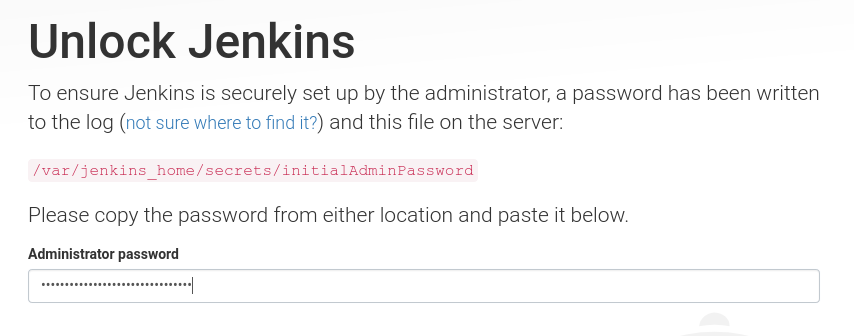
\includegraphics[width=0.6\textwidth]{imagens/i1Unlock.png}
	\caption{Solicitação do Token}
\end{figure}

Instalar os plugins sugeridos:
\begin{figure}[H]
	\centering
	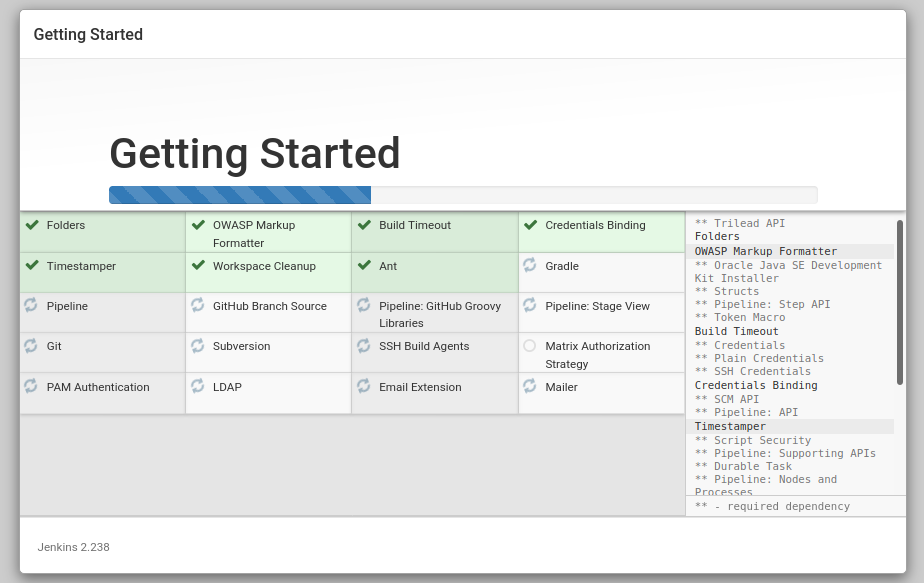
\includegraphics[width=0.6\textwidth]{imagens/i2Plugins.png}
	\caption{Instalação dos plugins}
\end{figure}

Escolher o usuário e senha, algo bem secreto como admin|admin:
\begin{figure}[H]
	\centering
	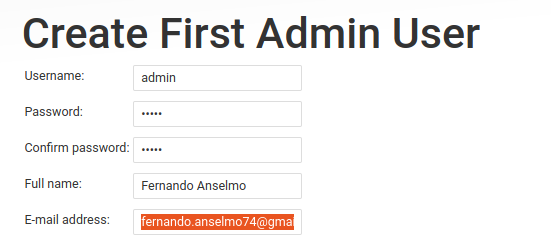
\includegraphics[width=0.6\textwidth]{imagens/i3CriarSenha.png}
	\caption{Criação do Usuário e Senha}
\end{figure}

Informar a URL do Jenkins e clicar no botão "Salvar e Finalizar":
\begin{figure}[H]
	\centering
	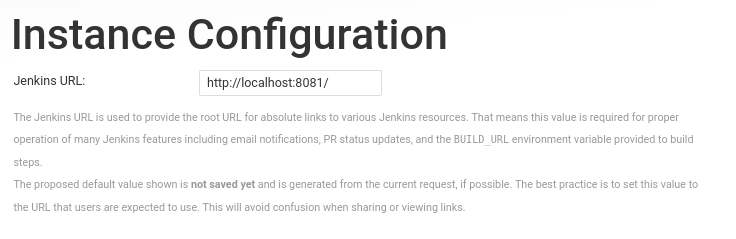
\includegraphics[width=0.6\textwidth]{imagens/i4ConfirmaUrl.png}
	\caption{Criação do Usuário e Senha}
\end{figure}

Parabéns o Jenkins foi instalado com sucesso.
\begin{figure}[H]
	\centering
	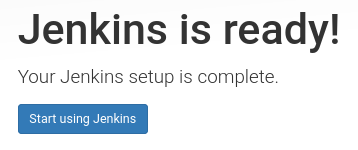
\includegraphics[width=0.6\textwidth]{imagens/i5Parabens.png}
	\caption{Criação do Usuário e Senha}
\end{figure}

\section{Entrar no Jenkins}
Algumas vezes precisamos de algumas informações relacionadas a máquina do Jenkins, então precisamos acessá-lo, no contêiner podemos fazer isso através do comando: //
\codigo{\$ docker exec -it meu-jenkins /bin/bash}

E estaremos dentro deste, podemos ver a versão do sistema:
\codigo{\$ cat /etc/os-release}

para sair digitamos o comando:
\codigo{\$ exit}

Este comando lista todos os contêineres que estão ativos:
\codigo{\$ docker container ls}

Observamos que cada contêiner possui um \textbf{CONTAINER ID}, este é usado, por exemplo para realizar uma inspeção de alguns detalhes deste:
\codigo{\$ docker container inspect [CONTAINER ID]}

\subsection{Para atualizar o Jenkins no Docker}
Atualizações de plugins no Jenkins podem ser realizadas direto no "Gerenciador do Jenkins", porém quando este informar que existe uma nova versão disponível, não é necessário baixá-la, apenas copiar o link do arquivo jenkins.war e proceder da seguinte forma:

Entrar no container do Jenkins: \\
\codigo{\$ docker exec -u 0 -it meu-jenkins bash}

Baixar a última versão: \\
\codigo{\$ wget [link do jenkins.war]}

Mover para o local correto: \\
\codigo{\$ mv ./jenkins.war /usr/share/jenkins}

Mudar a permissão: \\
\codigo{\$ chown jenkins:jenkins /usr/share/jenkins/jenkins.war}

Sair do bash: \\
\codigo{\$ exit}

Reiniciar o container: \\
\codigo{\$ docker restart meu-jenkins}

\section{Pipelines}
Como já dissemos, um \textit{pipeline} nada mais é do que uma sequencia de comandos que o Jenkins executará. A partir da versão 2.0 eles tomaram como base os arquivos script do Groovy.
A documentação completa pode ser encontrada nesta URL \url{https://www.jenkins.io/doc/book/pipeline/syntax/}. Nesta apostila vamos ver alguns passos básicos para iniciarmos sem problemas. Por padrão possuem a seguinte estrutura:
\begin{lstlisting}
pipeline {
  agent any
  stages {
    stage('Descritivo') {
      steps {
        // comandos
      }
    }
    ...
  }
}
\end{lstlisting}

Um script pode possuir vários estágios (\textit{stage}) para executar e são sincronizados e dependentes, ou seja, não pode ocorrer erro no antecessor senão todo o processo será interrompido.

\subsection{Hello World}
Vamos criar um simples script para entendermos como esse conceito funciona. Na tela principal do Jenkins clicar em "New Item".

Na opção \textbf{Item Name} informamos \textbf{Hello World}. E escolhemos o modo \textbf{Pipeline}, e confirmamos ao clicar em \textbf{OK}.

Se já conhece o Jenkins notará que esta opção é bem simples e basicamente se concentra na seção \textbf{Pipeline} na qual escrevemos nosso script:
\begin{lstlisting}
pipeline {
  agent any
  stages {
    stage('Hello') {
      steps {
		echo 'Hello World'
      }
    }
  }
}
\end{lstlisting}

\textbf{Apply} pode ser utilizado para verificar se existe qualquer problema na sintaxe. E uma vez terminado clicar em \textbf{Save}.

Para executar o script clicar em \textbf{Build Now}. Neste momento o Jenkins agenda seu script para ser executado assim que existir um agente livre. Pense que vários deles podem estar em execução neste momento, se assim ocorrer, e para não sobrecarregar a máquina, o Jenkins trabalha com sincronização e destina um serviço. Essa quantidade de serviços rodando simultaneamente pode ser configurada no Gerenciador.

A seguinte tela será mostrada caso seu script rode corretamente:
\begin{figure}[H]
	\centering
	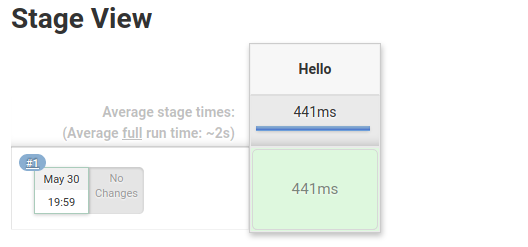
\includegraphics[width=0.6\textwidth]{imagens/scriptHW.png}
	\caption{Script Hello World executado com sucesso}
\end{figure}

Ao clicarmos nessa área verde uma opção para visualizar o LOG será mostrada e a nossa mensagem aparecerá.

\subsection{Hello World Docker}
Sabemos que o Docker possui uma imagem de teste chamada \textbf{hello-world} e vamos usá-la para testar se está tudo OK. Proceda os mesmos passos descritos anteriormente para criarmos um novo \textit{pipeline} chamado \textbf{Docker Hello} com o seguinte script:
\begin{lstlisting}
pipeline {
  agent any
  stages {
    stage("Baixar Imagem") {
      steps {
        sh 'docker pull hello-world'
      }
    }
    stage("Executar Hello") {
      steps {
        sh 'docker run hello-world'
      }
    }
  }
}
\end{lstlisting}

E assim o Jenkins envia um comando ao Docker da máquina hospedeira (não dentro do contêiner) para trazer a imagem \textbf{hello-world} do repositório Docker e em seguida criar um contêiner. Observamos que esses estágios são totalmente dependentes pois se não conseguir trazer a imagem não teria sentido de criar um contêiner.

Após sua execução vamos dar o seguinte comando na máquina local: \\
\codigo{\$ docker images}

Perceberemos agora a existência da imagem \textbf{hello-world} e o comando: \\
\codigo{\$ docker ps -a}

Observamos que agora possuímos um novo contêiner já parado. Vamos agora executar o mesmo processo, porém ao término de mostrar a mensagem eliminar tanto o contêiner quanto a imagem. 

Sabemos que para apagar um contêiner devemos dar o comando: \\
\codigo{\$ docker rm [Contêiner ID]}

E para apagarmos a imagem:
\codigo{\$ docker rmi [Imagem ID]}

Apague ambos manualmente para não deixar nenhuma trilha no seu Docker. Lembre-se que o Jenkins só vai fazer o que pediu, então partimos da premissa que devemos conhecer todos os comandos que o Jenkins executará. Primeiro passo será conhecer o comando para localizar o ID do contêiner: \\
\codigo{\$ docker ps -a --quiet --filter ancestor=[nome imagem]}

Que lista todos os IDs dos contêineres parados ou não (opção \codigo{ -a --quiet}) que pertencem a uma determinada imagem (opção ancestor do filter).

A segunda parte do problema e próximo passo está em localizar o ID da imagem criada, que é resolvido com o comando:
\codigo{\$ docker images [nome imagem] --quiet}

Que lista apenas o ID (opção \codigo{ --quiet}) de uma determinada imagem definida em [nome imagem].

Pronto, agora basta sabermos que no script podemos criar uma variável que armazena os IDs tanto do contêiner quanto da imagem para logo em seguida eliminá-los: \\
\codigo{ variável = sh(script: "[comando]", returnStdout: true).trim()}

Sendo assim, modificamos nosso script para:
\begin{lstlisting}
pipeline {
  agent any
  stages {
    stage("Baixar Imagem") {
      steps {
        sh 'docker pull hello-world'
      }
    }
    stage("Executar Hello") {
      steps {
        sh 'docker run hello-world'
      }
    }
    stage("Limpar") {
      steps {
        script {
          containerID = sh(script: "docker ps -a --quiet --filter ancestor=hello-world", returnStdout: true).trim()
          sh "docker rm ${containerID}"
          imagemID = sh(script: "docker images hello-world --quiet", returnStdout: true).trim()
          sh "docker rmi ${imagemID}"
        }
      }
    }        
  }
}
\end{lstlisting}

Observamos que ganhamos mais um estágio. Nesse novo as ações devem estar dentro de uma tag \textit{script} pois precisamos criar uma variável para conter nossos ID. Esse estágio "Limpar" poderia ser dividido em 2\footnote{Primeiro remove o Contêiner e em seguida a imagem.}, ou seja, a criação de estágios busca uma melhor organização para seu \textit{pipeline} e cabe ao Administrador resolver o resultado mais organizado\footnote{Compreenda que não existe uma receita de bolo.}.

\subsection{Obter parâmetros}
Parâmetros são essenciais para um pipeline, imaginemos que temos 4 ambientes: Desenvolvimento (DEV), Teste (TST), Homologação (HML) e Produção (PRD). Cada um desses ambientes define uma porta diferente para o Docker, uma solução seria criar 4 pipelines idênticos mudando somente o detalhe da porta (ou qualquer outro), porém devemos nos atentar na hora da manutenção e ter que corrigir erros em quatro pipelines (ao invés de um). Não seria então mais coerente criarmos um único pipeline e receber como parâmetro o ambiente?
\begin{lstlisting}
pipeline {
  agent any
  parameters {
    string(name: "COMMIT", defaultValue: "*/development", description: "Informe o CommitID")
    choice(name: "AMBIENTE", choices: ["DEV", "TST", "HML", "PRD"], description: "Ambiente a executar")
  }
  stages {
    stage("Execução") {
      steps {
        script {
          if (params.AMBIENTE.equals("DEV")) {
            PORTA = "8080"
          }  
          if (params.AMBIENTE.equals("TST")) {
            PORTA = "8081"
          }  
          if (params.AMBIENTE.equals("HML")) {
            PORTA = "8082"
          }  
          if (params.AMBIENTE.equals("PRD")) {
            PORTA = "8083"
          }
        }
        echo "Aqui os dados: ${params.COMMIT} e ${params.AMBIENTE}"
        echo "Pode usar assim: ${PORTA}"
        echo "Ou assim: " + PORTA
      }
    }
  }
}
\end{lstlisting}

Criamos para este pipeline dois parâmetros, o primeiro obtém o ID do Commit feito no GitHub (o último pode ser conseguido por "*/branch") e o segundo define em qual ambiente será executado. E se for, por exemplo, escolhido o ambiente de teste clicando na área verde temos:
\begin{figure}[H]
	\centering
	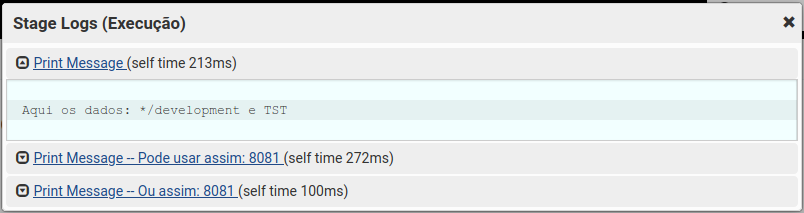
\includegraphics[width=0.5\textwidth]{imagens/parametro.png}
	\caption{Saída do Pipeline}
\end{figure}

Como este é um simples exemplo apenas mostramos no estágio o conteúdo dos parâmetros.

Um dado interessante: existe a opção "\textit{This project is parameterized}" e assim que for salvo esta opção conterá os dois parâmetros aqui descritos. Então qual a vantagem de se colocar no script? É assim que está definido na documentação, então para não ocorrermos no perigo de em próximas versões essa opção desaparecer já sabemos como proceder.

\subsection{Obter arquivos do Github}
Nossos arquivos devem estar em um local aonde o Jenkins poderá buscá-los e proceder os passos necessários para transformá-los no artefato final. Devemos pensar na seguinte situação:
\begin{figure}[H]
	\centering
	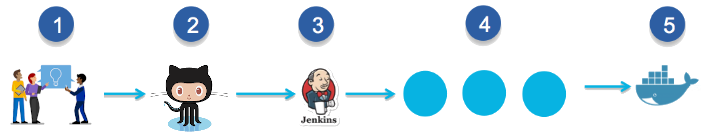
\includegraphics[width=1.0\textwidth]{imagens/cicloDev.png}
	\caption{Ciclo de Desenvolvimento}
\end{figure}

No \textbf{passo 1} os desenvolvedores planejam e discutem como será o artefato a ser realizado, no \textbf{passo 2} sobem os códigos fontes necessários ao projeto para o GitHub, no \textbf{passo 3} o Jenkins obtém esses códigos e começar a processar o \textit{pipeline} que está descrito no \textbf{passo 4} executando todos os processos necessários tais como compilação do código, execução do SonarQube para atestar a qualidade do que foi disponibilizado está de acordo com as diretrizes da Empresa e ao término, no \textbf{passo 5} cria a imagem e publica o contêiner.

Podemos ver que não existe qualquer mágica nesse processo, somente a automatização de modo que se não tivéssemos o Jenkins para realizá-los seria manual ou através do uso de qualquer outra ferramenta que trabalhe de modo similar como o Bamboo, Buildbot, Apache Gump ou o Travis CI que são seus concorrentes mais diretos.

Considerando que já possui uma conta no GitHub de Administrador ativa, devemos informar para o Jenkins criar uma credencial, para isso, a partir da tela principal devemos acessar \textbf{Credentials} $\triangleright$ \textbf{System} $\triangleright$ \textbf{Global credentials} e selecionar a propriedade \textbf{Add Credentials}.

Em \textbf{Username} informar o usuário administrador do repositório, em \textbf{Password} sua senha e em \textbf{Description} a que se refere (não preencha o campo \textbf{ID}) e quando pressionarmos o botão OK um ID será criado para este registro. Salve-o pois o utilizaremos no script para acessar o GitHub.
\begin{figure}[H]
	\centering
	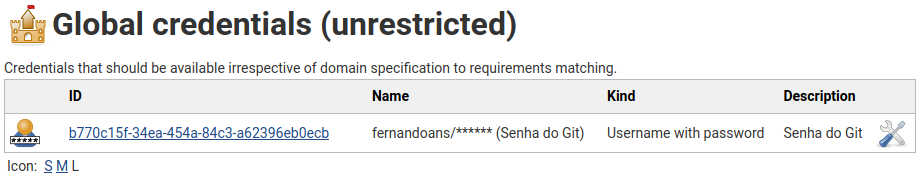
\includegraphics[width=1.0\textwidth]{imagens/credentials.png}
	\caption{Credencial criada}
\end{figure}

Observamos que na imagem a credencial criada para meu usuário. Não tem medo de mostrá-la? Não, pois só é acessível pelo meu Jenkins que associa este número ao meu usuário e a senha\footnote{Como podemos perceber está bem escondida, então não se preocupe.}. Ou seja, mesmo que saiba esse número não lhe servirá absolutamente para nada. Por isso o Jenkins mostra que é uma área não restrita.

\section{Criação de um projeto completo}
Podemos criar qualquer tipo de projeto e para tentar deixar bem simples aqui faremos um Projeto JSP que mostrará uma página, como dissemos a mesma ideia pode ser aplicada a qualquer projeto, então usemos esse somente como um ponto de partida.

\subsection{Construção do projeto}
Usamos o Spring Tool Suite\cite{sts} para criar o projeto. File $\triangleright$ New $\triangleright$ Project..., na janela que se abre procurar por Web $\triangleright$ Dynamic Web Project. Clicar no botão Next. Informar o nome do projeto (por Exemplo \textbf{tstJenkins}), não esquecer de modificar a opção "Use an environment JRE" para a versão correta da Java Runtime desejada e pressionar o botão Finish. Ao término pedirá para mudar a perspectiva da janela para a visão J2EE. Se está tudo correto teremos a seguinte situação na aba \textit{Project Explorer}:
\begin{figure}[H]
	\centering
	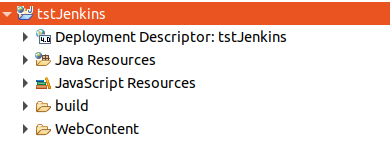
\includegraphics[width=0.4\textwidth]{imagens/projetoCriado.png}
	\caption{Projeto Decus criado}
\end{figure}

No projeto na pasta WebContent vamos criar um arquivo chamado "index.jsp" com o seguinte conteúdo:
\begin{lstlisting}
<%@page contentType="text/html; charset=UTF-8" pageEncoding="UTF-8"%>
<!DOCTYPE html>
<html lang="pt-BR">
<head>
 <title>Exemplo com Jenkins e Docker</title>
 <meta charset="UTF-8">
 <meta http-equiv="Content-Type" content="text/html; charset=UTF-8" />
</head>
<body>
 <h1 style="color:black">JSP publicado com Jenkins</h1>
 Essa aplicação utiliza o Jenkins para realizar uma publicação em 4 fases:
 <ul>
  <li>Obter os códigos no GitHub</li>
  <li>Gerar o arquivo WAR com o Maven</li>
  <li>Criar um contêiner em enviá-lo para o DockerHub</li>
  <li>Executar o contêiner da aplicação</li>
 </ul>
</body>
</html>
\end{lstlisting}

Sim, poderia ser também "index.html" visto que não existe um único código JSP aqui, porém como dissemos antes, use este para um ponto de partida para qualquer projeto que pode ser desde a criação de \textit{dashboard} para Análise de Dados até mesmo algo mais complexo. O objetivo desta apostila é mostrar os caminhos do Jenkins e não a concepção de projetos.

\subsection{Construção da Imagem para a Aplicação}
Sabemos que o Docker trabalha com imagens e o Jenkins necessita conhecer como é esse arquivo para poder gerá-la, na raiz do projeto devemos criar um arquivo chamado \textbf{Dockerfile}\footnote{Cuidado com as maiúsculas e minúsculas pois o nome deve ser exatamente este.} com o seguinte conteúdo:
\begin{lstlisting}
FROM tomcat:9
COPY target/*.war /usr/local/tomcat/webapps/tstJenkins.war
\end{lstlisting}

Como base usaremos a imagem do servidor \textbf{Apache TomCat 9}\footnote{Ou utilize outra de acordo com a configuração do servidor do seu projeto.} e colocamos o arquivo \textbf{war} (\textit{Web Archive}) no ponto correto para sua execução.

\subsection{Apache Maven}
O STS já é totalmente compatível com o Apache Maven\cite{maven} que é utilizado para a construção de todo o código então não precisamos nos preocupar muito com essa parte, porém o Jenkins precisa conhecer esse endereço, então devemos proceder sua instalação. Para isso basta baixar o arquivo compactado (apache-maven-3.6.3-bin.zip), descompactá-lo em uma pasta (a partir da raiz) e criar uma variável de ambiente chamada \textbf{mvnHome} de modo que podemos ter o acesso fácil a essa pasta.

Outro detalhe que precisamos é transformar o projeto para Maven de modo que o Jenkins possa realizar a compilação sem problemas. Clicar com o botão direito do mouse no projeto e acessar a opção: Configure $\triangleright$ Convert to Maven Project. Na janela apenas pressione o botão \textit{Finish}. Se tudo está correto observamos que o projeto ganhou uma letra \textbf{M} o que indica agora é um projeto padrão Maven. Então foi criado um arquivo chamado \textbf{pom.xml}.

Neste arquivo adicionar as seguintes dependências:
\begin{lstlisting}
<dependencies>
 <dependency>
  <groupId>javax.servlet</groupId>
  <artifactId>javax.servlet-api</artifactId>
  <version>3.0.1</version>
 </dependency>
 <dependency>
  <groupId>junit</groupId>
  <artifactId>junit</artifactId>
  <version>3.8.1</version>
  <scope>test</scope>
 </dependency>
</dependencies>
\end{lstlisting}

A primeira informa ao Maven que é um projeto JavaWeb e a segunda que deve ser adicionado o JUnit para a realização de testes unitários, é ideal que o Desenvolvedor se preocupe em garantir que todo o código entregue estará testado e funcionando para isso é essencial a implementação dos testes unitários.

\subsection{GitHub}
Obviamente precisamos de uma conta no GitHub para compartilhar o projeto (ou outro gerenciador de código). Clicar com o botão direito do mouse no projeto e acessar a opção: Team $\triangleright$ Share Project. Marcar a opção \textit{Use or create repository in parent folder of project} e pressionar o botão \textbf{Create Repository}. Por fim o botão \textit{Finish}.

Na perspectiva do Git é possível gerenciar todas as subidas e descidas para o repositório.

\subsection{SonarQube}
Com esta parte concluída podemos partir para a última fase, com o passar do tempo a complexidade do código tende a crescer, a realização de refatorações são sempre necessárias. Devemos nos preocupar em resolver os problemas de negócios, porém deixamos passar pequenos erros no código. Para resolver problemas como esses devemos utilizar ferramentas que nos auxiliem na análise do código produzido.

O SonarQube é uma plataforma de código aberto para inspeção contínua da qualidade deste, para executar revisões automáticas com análise estática como forma de encontrar problemas, erros e vulnerabilidades de segurança que pode ser usado em mais de 20 linguagens de programação. Lembre-se que para usar essa funcionalidade no Jenkins o plug=in \textbf{SonarQube Scanner} deve estar instalado corretamente.

Baixar a imagem oficial: \\
\codigo{\$ docker pull sonarqube}

Criar o contêiner: \\
\codigo{\$ docker run -d --name meu-sonar -p 9000:9000 -p 9092:9092 sonarqube}

Acessar o SonarQube na URL \url{http:\\localhost:9000} com usuário e senha admin|admin. E deve ser aberta a seguinte janela:
\begin{figure}[H]
	\centering
	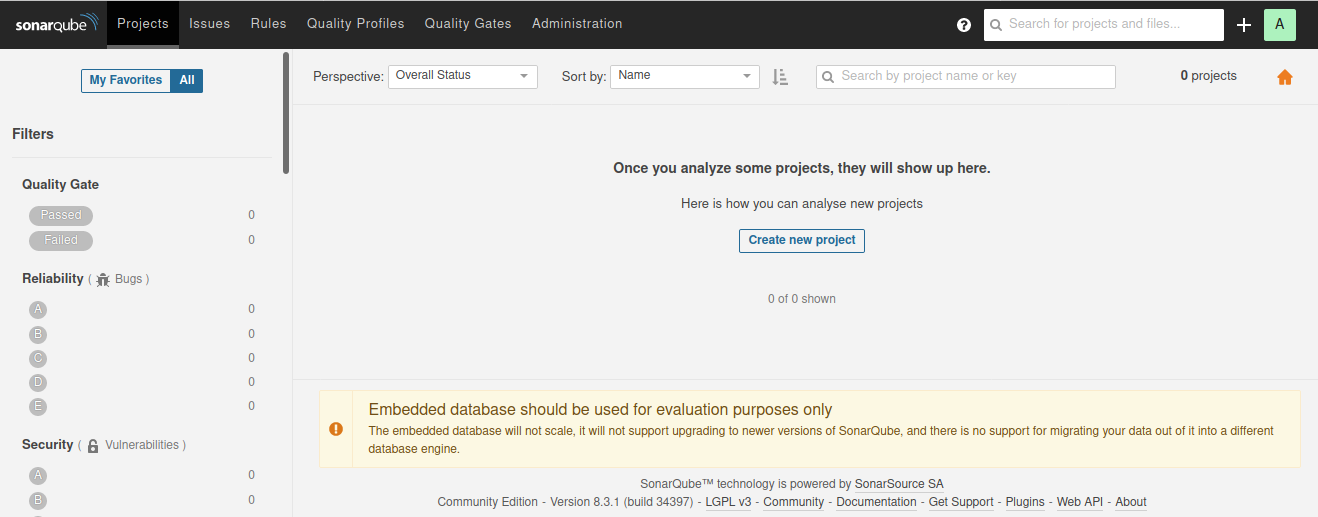
\includegraphics[width=0.8\textwidth]{imagens/sonar.png}
	\caption{Janela principal do SonarQube}
\end{figure}

O botão \textit{Create new project}. Ao clicar neste a solicitação para a chave do projeto, no qual podemos colocar o mesmo nome do projeto: tstJenkins. Assim fica mais fácil a sua localização. Em seguida a geração do Token, informar \textbf{meuToken}\footnote{Esse será salvo na seção do Administrador e pode ser usado por outros projetos - Guarde-o pois esse número NÃO SERÁ MAIS VISUALIZADO.} e clicar no botão \textit{Generate} e será gerado um código. Guardamos esse pois será necessário para o Jenkins.

Porém não usaremos tal funcionalidade para o Jenkins pois este exige outras configurações na qual recomendo consultar a documentação para verificar como proceder. Aqui manteremos as coisas simples, o STS possui o executor de comandos do Maven. Sendo que a meta completa que usaremos é a seguinte: \\
\codigo{\$ sonar:sonar -Dsonar.host.url=http://localhost:9000 \\ 
	-Dsonar.login=[numero do seu TOKEN] -Dsonar-projectName=tstJenkins \\
	-Dsonar.projectVersion=master}

Basta clicar com o botão direito no projeto e executar a Opção \textbf{Run As...}:
\begin{figure}[H]
	\centering
	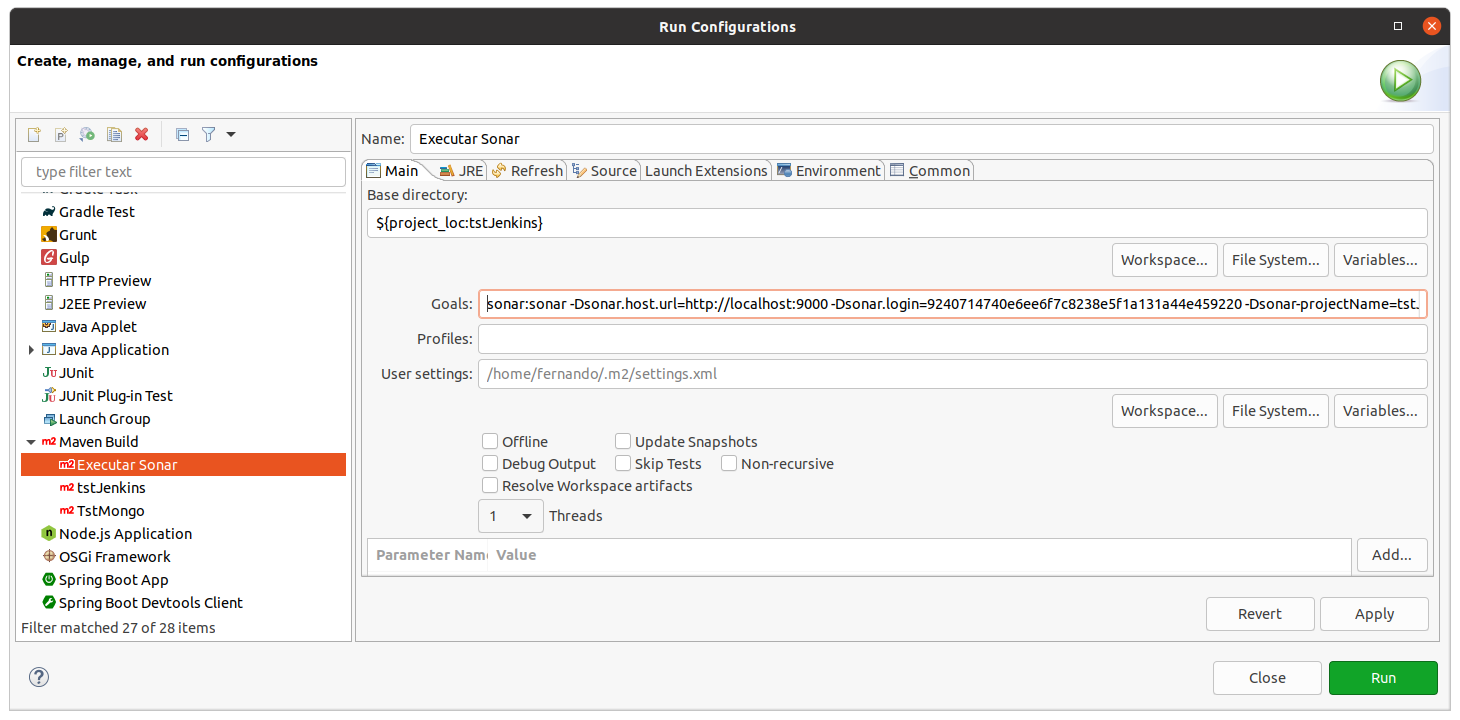
\includegraphics[width=0.8\textwidth]{imagens/sonarSTS.png}
	\caption{Janela principal do SonarQube}
\end{figure}

\subsection{Pipeline Final}
Com tudo posto podemos criar a seguinte pipeline:
\begin{lstlisting}
pipeline {
 agent any
 stages {
  stage('Verificar Credenciais Git') {
   steps {
    git credentialsId: '[credencial]', url: 'https://github.com/fernandoans/tstJenkins'
   }
  }
  stage('construir') {
   steps {
    script {
     def mvnHome = tool name: 'Maven3', type: 'maven'
     def mvnCMD = "${mvnHome}/bin/mvn"
     sh "${mvnCMD} clean package"
    }
   }
  }  
  stage('Construir Imagem Docker') {
   steps {
    script {
     sh 'docker build -t fernandoanselmo/meu-proj:1.0.0 .'
    }
   }
  }  
  stage('Subir a Imagem') {
   steps {
    script {
     withCredentials([string(credentialsId: 'DockerHubPwd', variable: 'DockerHub')]) {
      sh "docker login -u fernandoanselmo -p ${DockerHub}"
     }
     sh 'docker push fernandoanselmo/meu-proj:1.0.0'
    }
   }
  }
  stage('Executar Local') {
   steps {
	script {
     containerID = sh(script: "docker ps --quiet --filter name=meu-proj", returnStdout: true).trim()
     containerID = sh(script: "docker ps -a --quiet --filter name=meu-proj", returnStdout: true).trim()
     if (!containerID.isEmpty()) {
      sh 'docker stop meu-proj'
     }
     if (!containerID.isEmpty()) {
      sh 'docker rm meu-proj'
     }
     sh 'docker run -p 8080:8080 -d --name meu-proj fernandoanselmo/meu-proj:1.0.0'
    }
   }
  }
 }
}
\end{lstlisting}

E como resultado final obtemos a seguinte imagem:
\begin{figure}[H]
	\centering
	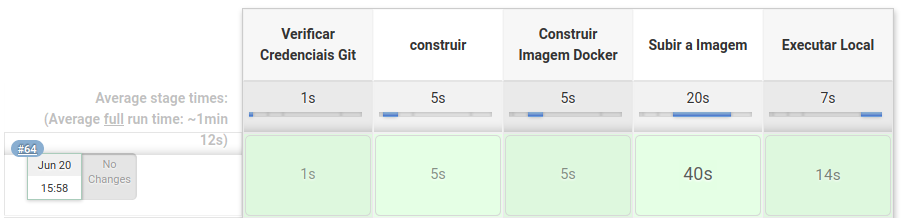
\includegraphics[width=0.8\textwidth]{imagens/pipelineFinal.png}
	\caption{Pipeline Final}
\end{figure}

E ao acessar o endereço \url{http://localhost:8080/tstJenkins/} teremos uma tela como esta:
\begin{figure}[H]
	\centering
	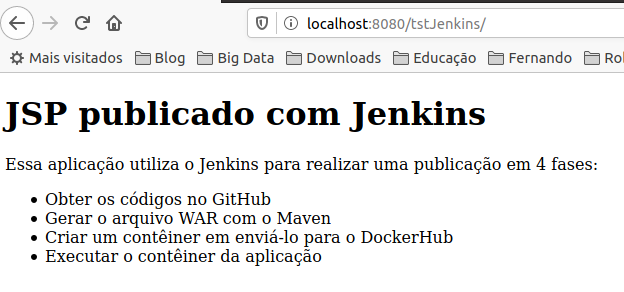
\includegraphics[width=0.6\textwidth]{imagens/projetoCompleto.png}
	\caption{Pipeline Final}
\end{figure}

\section{Conclusão}
O conceito de CD/CI surgiu para remover os problemas de localizar ocorrências posteriores no ciclo de vida da construção e que os desenvolvedores que integram o código em um repositório compartilhado em intervalos regulares possam ter a garantia que o mesmo estará em produção sem a interferência de falhas humanas na publicação. 

A automação de compilações e testes, melhora drasticamente os ciclos de lançamento de novos artefatos. À medida que cresce, o setor criou um ciclo contínuo para as implantações de produção. Jenkins permite passar do check-in do código à implantação de uma nova versão do nosso aplicativo na produção sem causar qualquer estresse uma vez que todo processo foi checado e validado. Assim os desenvolvedores podem integrar facilmente as alterações de aplicativos com essa ferramenta para ajudar o usuário a obter uma nova versão. 

Jenkins permite que o software seja testado e entregue continuamente com a ajuda de várias tecnologias de integração e implantação. Seus plugins nos ajudam a fornecer CD/CI em vários estágios diferentes e podem integrar qualquer ferramenta específica, como Git, Amazon EC2 ou Maven. 

Sou um entusiasta do mundo \textbf{Open Source} e novas tecnologias. Qual a diferença entre Livre e Open Source? \underline{Livre} significa que esta apostila é gratuita e pode ser compartilhada a vontade. \underline{Open Source} além de livre todos os arquivos que permitem a geração desta (chamados de arquivos fontes) devem ser disponibilizados para que qualquer pessoa possa modificar ao seu prazer, gerar novas, complementar ou fazer o que quiser. Os fontes da apostila (que foi produzida com o LaTex) está disponibilizado no GitHub \cite{github}. Veja ainda outros artigos que publico sobre tecnologia através do meu Blog Oficial \cite{fernandoanselmo}.

%-----------------------------------------------------------------------------
% REFERÊNCIAS
%-----------------------------------------------------------------------------
\begin{thebibliography}{7}
  \bibitem{jenkins} 
  Site oficial do Jenkins \\
  \url{https://www.jenkins.io/}

  \bibitem{sts} 
  Editor Spring Tool Suite para códigos Java \\
  \url{https://spring.io/tools}
  
  \bibitem{maven} 
  Apache Maven \\
  \url{https://maven.apache.org/}

  \bibitem{sonar} 
  SonarQube \\
  \url{https://www.sonarqube.org/}

  	\bibitem{fernandoanselmo} 
	Fernando Anselmo - Blog Oficial de Tecnologia \\
	\url{http://www.fernandoanselmo.blogspot.com.br/}
	
	\bibitem{publicacao} 
	Encontre essa e outras publicações em \\
	\url{https://cetrex.academia.edu/FernandoAnselmo}
	
	\bibitem{github} 
	Repositório para os fontes da apostila \\
	\url{https://github.com/fernandoans/publicacoes}
\end{thebibliography}

\end{document}
